\subsubsection{Web Browser Benchmark}
\label{sec:wbbench}

\begin{figure*}[htb]
\begin{center}
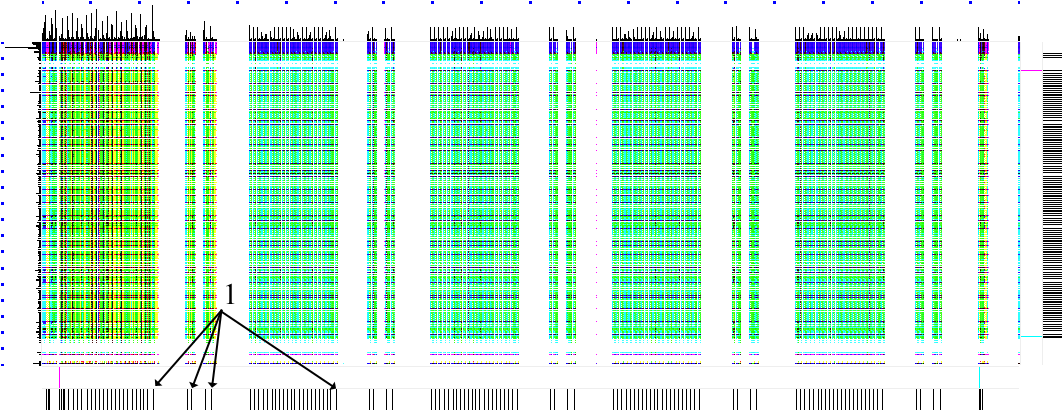
\includegraphics[width=0.7\textwidth]{lviz/wbbench-dp.png}
\end{center}
\caption{Time-ordered \VDP{} comparing IE7 (x-axis) and Chrome (y-axis)
performing the
SunSpider JavaScript benchmark.
}
\label{fig:wbbench-dp}
%\begin{tabular}{ll}
%DP match : & operation\\
%DP color : & cyan $\rightarrow$ file; magenta $\rightarrow$ registry;
%yellow $\rightarrow$ network operation\\
%Bar1 color : & cyan $\rightarrow$ benchmark start time;
%magenta $\rightarrow$ benchmark end time\\
%Bar2 color : & black $\rightarrow$ HTTP GET event
%\end{tabular}
{\it DP match}: operation;
{\it DP color}: cyan $\rightarrow$ file; magenta $\rightarrow$ registry;
yellow $\rightarrow$ network operation;
{\it Bar1 color}: cyan $\rightarrow$ benchmark start time;
magenta $\rightarrow$ benchmark end time;
{\it Bar2 color}: black $\rightarrow$ HTTP GET event.
\end{figure*}

We use time-ordered \VDP{} (Fig.~\ref{fig:wbbench-dp}) to investigate the
SunSpider JavaScript benchmarks on
two web browsers, Internet Explorer 7 (IE7) and Google Chrome.
The benchmark consists of 26 different tests repeated for 5 times.
Since the browser fetches a web page for each test,
we use the HTTP GET\footnote{
To mark HTTP GET events, we need to turn on network data I/O collection
and use a suitable regular expression as the barcode coloring rule.
The start and end events are marked by matching the two URLs.
}
event (shown in Bar2) to mark the beginning
of each test.
By looking at the time-ordered DP, we know that Chrome is about three
times faster than IE7 in total and also in each test.
From Bar2,
we can also observe that some tests (followed by long white gap,
pointed by marker 1) take much longer time than others.
By clicking on those events, we found out the slow ones to be all string
operation\footnote{
The URLs are \url{/perf/sunspider-0.9/string-base64.html},
\url{/perf/sunspider-0.9/string-tagcloud.html},
and \url{/perf/sunspider-0.9/string-validate-input.html}}
benchmarks.
We conclude that one reason why IE7 is slower than Chrome is due to string operations.
